%===============================================================================
% $Id: ifacconf.tex 19 2011-10-27 09:32:13Z jpuente $  
% Template for IFAC meeting papers
% Copyright (c) 2007-2008 International Federation of Automatic Control
%===============================================================================
\documentclass[a4paper]{ifacconf}

\usepackage{graphicx,amsmath,url}      % include this line if your document contains figures
\usepackage[round]{natbib}             % required for bibliography
%===============================================================================


% ===============================================================
% Choose the language of the manuscript.
% If in English, choose 
% \def\portugues{0} 
%
% If in Portuguese or Spanish, choose
% \def\portugues{1} 
%
% Note that, if you are writing in Spanish, you need additional 
% adjusts in some parts of the text, which have been put in Portuguese only.
\def\portugues{1} 
% ===============================================================

% If the above line is commented, it is assumed manuscript in English:
\ifx\portugues\undefined
\def\portugues{0}
\fi


\if\portugues0
   \usepackage[english]{babel}
  \else
   \usepackage[spanish,brazil,english]{babel}
\fi

  

\usepackage[T1]{fontenc}
%\usepackage{inputenc}

\usepackage[utf8]{inputenc}

\usepackage{ae}


\if\portugues1
% =====================================================================
% =====================================================================
% If the manuscript is in Spanish, please change the texts adequatelly.
% You may also add other definitions in this part.
 \newtheorem{teorema}[thm]{{\em Teorema}}{ }
 \newtheorem{lema}[thm]{{\em Lema}}{ }
 \newtheorem{corolario}[thm]{{\em Corolário}}{ }
 \newenvironment{prova}{{\bf Prova.}}{ }
% ===============================================================
\fi

\begin{document}
	
	
\if\portugues1

% =====================================================================
% =====================================================================
% USE THIS PART IF THE TEXT IS IN PORTUGUES OR SPANISH
% =====================================================================
% If the manuscript is in Spanish, please change the texts adequately.
% =====================================================================
% 
\selectlanguage{brazil}
	
\begin{frontmatter}

\title{Reciclagem Digital: resignificando o lixo eletrônico na comunidade ouropretana}
%Do lixo à sala de aula: uma experiência educativa com o programa Reciclagem Digital --> podemos pensar num título mais atraente!

\author[1]{Danny A.V. Tonidandel}
\author[1]{Adrielle C. Santana}
\author[1]{Regiane S.S. Ramalho}
\author[2]{Cristiano L.T.F. Silva}

\address[1]{Universidade Federal de Ouro Preto (UFOP)\\ Departamento de Eng. de Controle $\&$ Automação \\ Ouro Preto, MG, Brasil, (e-mails: tonidandel@ufop.edu.br, adrielle@ufop.edu.br, regiane@ufop.edu.br).}

\address[2]{Universidade Federal de Ouro Preto\\ Departamento de Eng. de Produção \\ Ouro Preto, MG, Brasil, (e-mail: cristiano.silva@ufop.edu.br)}


\selectlanguage{english}
\renewcommand{\abstractname}{{\bf Abstract:~}}
\begin{abstract}                % Abstract of not more than 250 words.
According with information from ONU, the trash from computer systems as, computers and cellphones, grows at a rate around three times greater than that from the common trash. In just over $60$ years after the emergence of computers around the world, in that the obsolescence from systems $-$ stimulated by the market economy $-$ is increasingly precocious, the amount of trash generated from compunents still in condition for use is practically incalculable, as well as the negative environmental impact that will be converted in a heavy weight for future generations. The electronic junk have dozens of contaminants and, even if discarded in a correct way, can provoke a lot of damage to the environment. Between the ways to deal with such a movement, it was created the University Extension program ``Reciclagem Digital'' that encompassed actions of computers refurbishment and update (\emph{Hospital das Máquinas project}), assembly of computers from electronic junk (\emph{Frankenstein project}) and the reuse of electronic components (\emph{Manufatura Reversa project}) from damaged electronics of the University and also the community. Idealized by teachers from the Control and Automation Engineering and Production Engineering courses from the Universidade Federal de Ouro Preto, the Recicalgem Digital program was one of the success actions to mitigate the environmental impact provokedd by the electronic junk. This paper present a experiences report from this educationsl program, accomplished along the years of $2016$ to $2018$.

\vskip 1mm% não altere esse espaçamento
\selectlanguage{brazil}
{\noindent \bf Resumo}:  Segundo informações ONU, o lixo proveniente de sistemas computacionais, como computadores e celulares, cresce a uma taxa cerca de três vezes maior que a do lixo comum. Em pouco mais de $60$ anos após a aparição dos computadores no mundo, em que a obsolescência dos sistemas $-$ estimulada pela economia de mercado $-$ é cada vez mais precoce, a quantidade de lixo gerada a partir de componentes ainda em condições de uso é praticamente incalculável, assim como o impacto ambiental negativo que se converterá em pesado fardo para as gerações futuras. O lixo eletrônico contém dezenas de contaminantes e, mesmo descartados de maneira correta, podem provocar muitos danos ao meio ambiente. Entre as alternativas para se deter tal movimento, foi criado o programa de Extensão Universitária ``Reciclagem Digital'' que englobava ações de reforma e atualização de computadores (\emph{projeto Hospital das Máquinas}), montagem de computadores a partir do lixo eletrônico (\emph{projeto Frankenstein}) e no aproveitamento de componentes eletrônicos (\emph{projeto Manufatura Reversa}) a partir de eletroeletrônicos defeituosos na Universidade e na comunidade. Idealizado por professores dos cursos de Engenharia de Controle e Automação e Engenharia de Produção da Universidade Federal de Ouro preto, o programa Reciclagem Digital foi uma das ações de sucesso em mitigar o impacto ambiental provocado pelo lixo eletrônico. Este artigo apresenta um relato de experiências desse programa educativo, realizado ao longo dos anos de $2016$ a $2018$.
\end{abstract}

\selectlanguage{english}
\begin{keyword}
Electronic Junk, Electronic Components, Recycling, Environment and Computers.

\vskip 1mm% não altere esse espaçamento
\selectlanguage{brazil}
{\noindent\it Palavras-chaves:} Lixo Eletrônico, Componentes Eletrônicos, Reciclagem, Meio Ambiente e Computadores.
\end{keyword}

\selectlanguage{brazil}

\end{frontmatter}


%===============================================================================
%===============================================================================
%===============================================================================


\section{Introdução}


É praticamente impossível mensurar o tesouro que está sob nossos pés. E não estamos falando de minério ou outro recurso natural: trata-se do lixo eletrônico, e-lixo ou, da silga em inglês E-waste. Dados oficiais das Naçoes Unidas\footnote{Uma delas é o observatório Global E-waste, disponível em {http://ewastemonitor.info/}.} indicam que, até o ano de $2017$, mais de $1,5$ milhões de toneladas de lixo eletrônico $-$ aqueles oriundos de placas de circuito, monitores de computador, celulares e eletrodomésticos  $-$ eram produzidos apenas no Brasil, perdendo para os EUA, que geraram até este ano, mais de $6$ milhões de toneladas. No mundo, estima-se que esta marca ultrapasse os $50$ milhões produzidos todo ano.\\

Boa parte do lixo eletrônico pode ainda gerar renda. Muitos componentes eletrônicos como placas de circuitos integrados, memórias e processadores, são também formados por elementos preciosos como ouro e prata \citep{Salviato}. Além disso, diversos componentes podem ainda ser reaproveitados pois, muitas vezes, um equipamento inteiro é descartado pelo mau funcionamento de apenas um ou alguns poucos componentes. Nesses casos, tanto a substituição dos componentes defeituosos como a retirada dos componentes bons para uso em outros equipamentos pode ser feita, reduzindo, assim, a quantidade do lixo eletrônico gerado. Infelizmente apenas $2\%$ do lixo eletrônico brasileiro é reciclado o que é um grande desperdício pois, segundo o Ministério do Meio Ambiente, a reciclagem dos resíduos eletrônicos poderia gerar até dez mil empregos e $R\$700$ milhões em recursos \citep{Salviato}. \\

Observando o crescente acúmulo de lixo eletrônico na Universidade Federal de Ouro Preto (UFOP), a necessidade de fomentar a inclusão digital nas instituições de ensino mais carentes da sociedade ouropretana e a necessidade constante de componentes específicos para aulas e experimentos dos diversos cursos da UFOP que não são rapidamente adquiridos pela administração, o programa Reciclagem Digital surgiu como uma tentativa de sanar tais problemas.

Desde o início, foi acertado que o objetivo do programa era, em essência, trabalhar pelo acesso às tecnologias digitais para uma maior inclusão social e educação: seja com o fornecimento de computadores, sua manutenção ou, simplesmente, pela retirada do lixo eletrônico e seu correto descarte. O programa era de caráter educativo tanto na área socioambiental quanto econômica, pois visava prolongar a vida útil dos equipamentos que seriam descartados ou considerados ``obsoletos''.\\

O programa Reciclagem Digital agregou ações que visavam a diminuição do impacto ambiental provocado pelo lixo eletrônico que se desdobrou em várias frentes: manutenção de computadores da comunidade, doação de PC's montados a partir do lixo eletrônico coletado e aproveitamento de material eletrônico para atividades de ensino e pesquisa na UFOP.\\

\section{Estruturação do Programa}

A ideia do primeiro projeto surgiu a partir de uma demanda por computadores para o laboratório de Instrumentação e Metrologia do Departamento de Engenharia de Controle e Automação da UFOP. Na ocasião, após uma conversa entre professores e estudantes voluntários, foi combinada uma visita ao setor de desfazimento da universidade. Lá observamos uma grande quantidade de peças e sistemas computacionais que estavam com o status de ``obsoletos'' ou ``defeituosos''. A visão era impactante: pilhas e mais pilhas de computadores, monitores, teclados e impressoras, que tinham apenas o lixo como destino. No entanto, observamos que diversos componentes eletrônicos, desde placas de circuitos, monitores e CPU's poderiam ser reaproveitados, não apenas para o laboratório, mas para auxiliar outras pessoas. Alguns dias depois, tendo em mente que um dos objetivos da universidade pública é contribuir para o desenvolvimento material e cultural da comunidade, pensou-se que do ``lixo'' pudessem surgir algumas ações, que foram nomeadas de acordo com seus propósitos principais: Hospital das Máquinas, Frankenstein e Manufatura Reversa, que integraram o programa \emph{Reciclagem Digital}.\\

O programa foi aprovado pela Pró-Reitoria de Extensão da UFOP \citep{proex} no primeiro semestre de 2016 com 3 bolsas para alunos UFOP. No entanto, mais dois alunos se juntaram ao projeto de forma voluntária, interessados não somente em adquirir experiência como colaborar com a causa do programa. A partir daí, um espaço físico para os alunos trabalharem foi providenciado, ferramentas básicas foram adquiridas pelos professores com recursos próprios e o programa começou efetivamente a funcionar.

A seguir, cada ação (projeto) do programa Reciclagem Digital é detalhada bem como os desafios enfrentados no decorrer das atividades.

\subsection{Hospital das Máquinas}

Manutenção de computadores da comunidade

\subsection{Frankenstein}

Reforma e atualização de computadores montados a partir do lixo eletrônico do setor de desfazimento da UFOP ou material coletado na comunidade.

\subsection{Manufatura Reversa}

aproveitamento de equipamento e material eletrônico para atividades de ensino e pesquisa na UFOP

\section{Resultados}

\subsection{Hospital das Máquinas}

\begin{figure}
\begin{center}
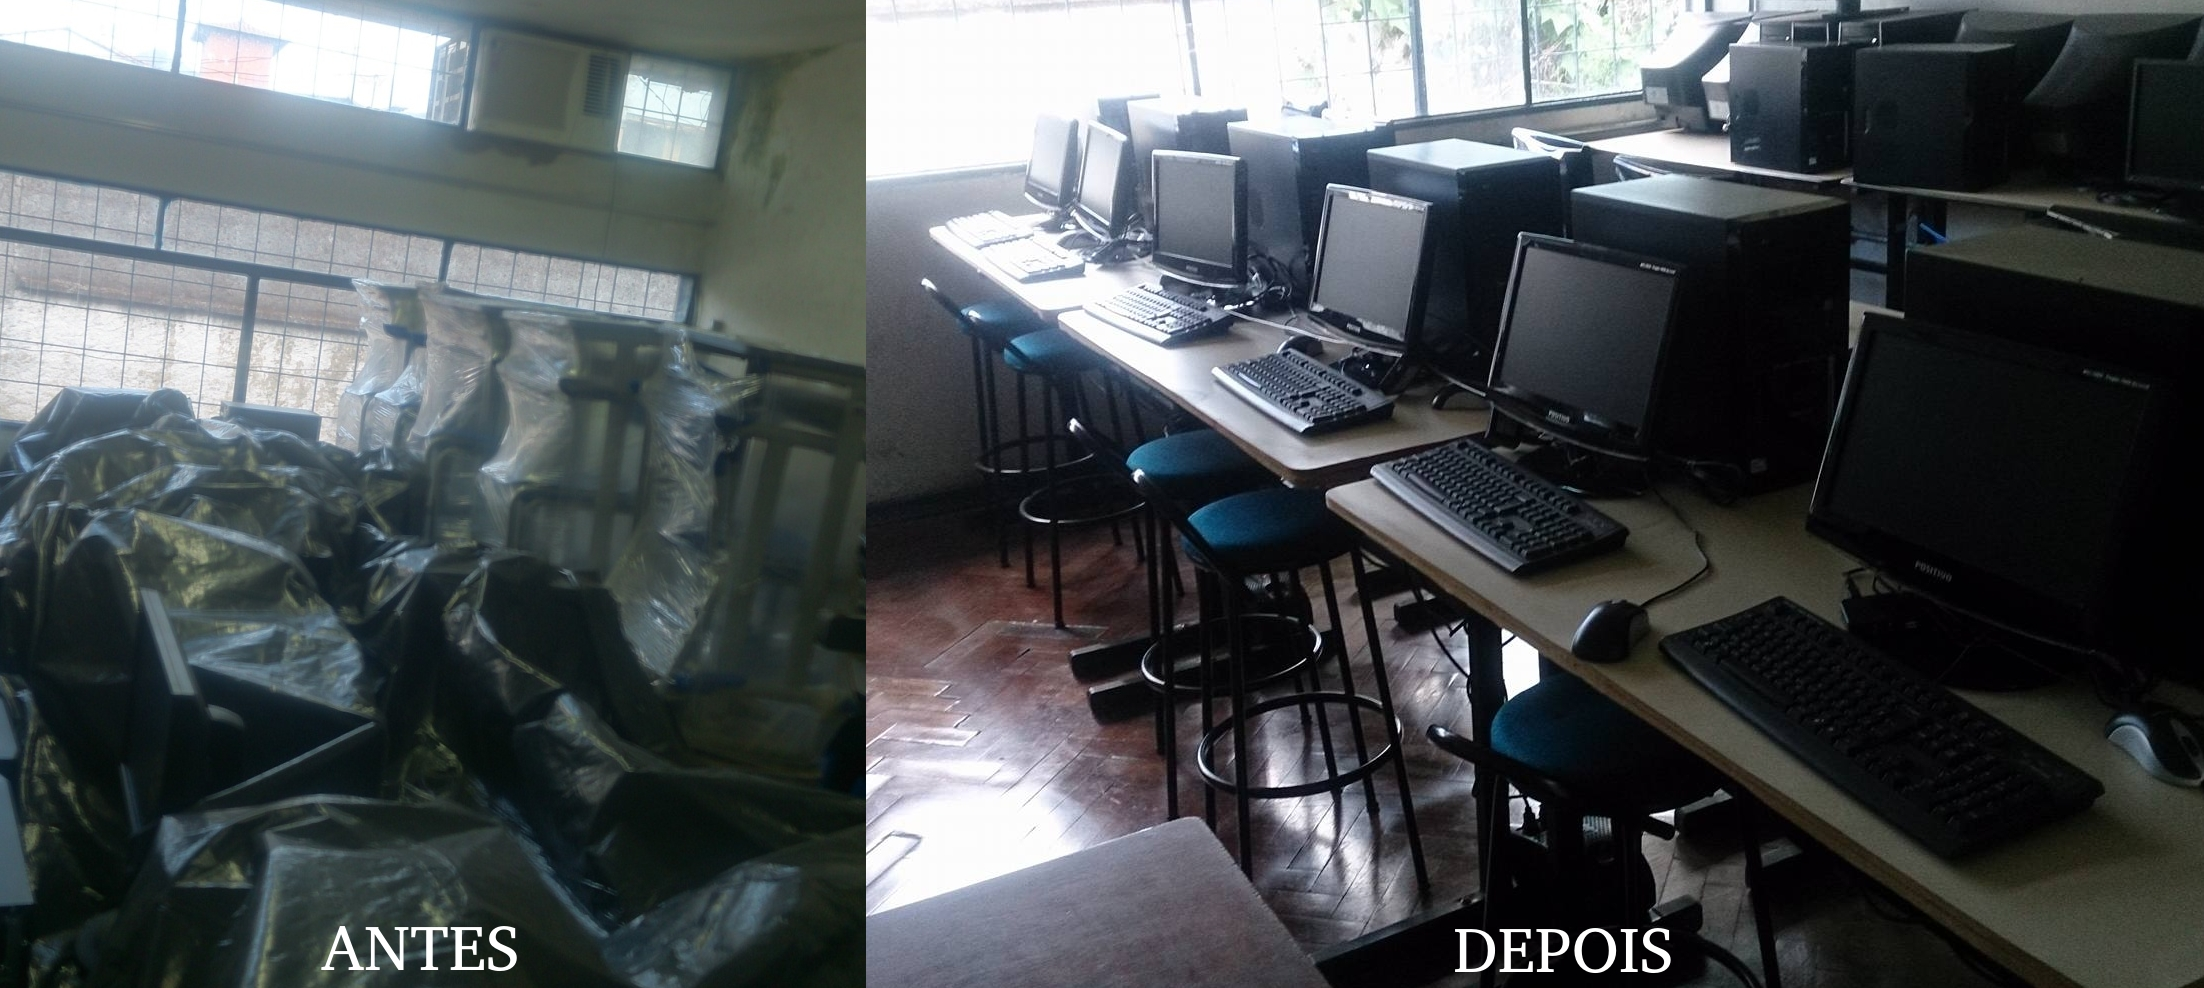
\includegraphics[width=8.4cm]{Figuras/2016-ee-dom-silverio-antes-depois.jpg}    
\caption{Laboratório de Computação da Escola Estadual Dom Silvério: antes e depois.} 
\label{fig:bifurcation}
\end{center}
\end{figure}

\subsection{Frankestein}

\subsection{Manufatura Reversa}



Tabelas devem ser centralizadas, ter uma legenda acima e ser numeradas em arábicos.


\section{Conclusão}

Uma seção com a conclusão não é obrigatória. 

\section*{Agradecimentos}
Os autores agradecem à PROEX que acreditou no programa e forneceu as bolsas necessárias aos alunos. Agradecemos sinceramente aos alunos bolsistas e voluntários que possibilitaram a execução do programa Reciclagem Digital a citar: Gabriel V. R. Hoffman, Brian A. Fernandes, Jonisson S. Santos, Heitor A. De Novais, Aluizio J. Grecco, Dauberson Alves Mol, Hamilton Tonidandel Junior, Francisco de Sales Gregorio Neto, Thiago Vilela Pena, Luciano E. de Almeida e Ciro Limão.

\bibliography{ifacconf}                                                                  

\end{document}
